% begin module diff-eq-natural-growth-solution
\begin{frame}
\begin{columns}[c]
\column{.4\textwidth}
\[
\frac{\diff P}{\diff t} = k P
\]
\column{.6\textwidth}
\psset{xunit=0.5cm, yunit=0.5cm}
\begin{pspicture}(-2.200000, -3.836002)(2.200000,3.836002)
\tiny
\fcAxesStandard{-2.000000}{-3.686002}{2.000000}{3.636002}
\uncover<10>{
%Function formula: -1/5 e^{x}
\psplot[linecolor=\fcColorGraph, plotpoints=1000]{-2.000000}{2.000000}{2.718281828 x exp -0.2000000 mul }
%Function formula: -1/2 e^{x}
\psplot[linecolor=blue, plotpoints=1000]{-2.000000}{2.000000}{2.718281828 x exp -0.5000000 mul }
%Function formula: -2/5 e^{x}
\psplot[linecolor=cyan, plotpoints=1000]{-2.000000}{2.000000}{2.718281828 x exp -0.4000000 mul }
%Function formula: -3/10 e^{x}
\psplot[linecolor=brown, plotpoints=1000]{-2.000000}{2.000000}{2.718281828 x exp -0.3000000 mul }
}
\uncover<10->{%
%Function formula: 3/10 e^{x}
\psplot[linecolor=orange, plotpoints=1000]{-2.000000}{2.000000}{2.718281828 x exp 0.3000000 mul }
%Function formula: 2/5 e^{x}
\psplot[linecolor=magenta, plotpoints=1000]{-2.000000}{2.000000}{2.718281828 x exp 0.4000000 mul }
%Function formula: 1/2 e^{x}
\psplot[linecolor=green, plotpoints=1000]{-2.000000}{2.000000}{2.718281828 x exp 0.5000000 mul }
%Function formula: 1/5 e^{x}
\psplot[linecolor=red, plotpoints=1000]{-2.000000}{2.000000}{2.718281828 x exp 0.2000000 mul }
}
\end{pspicture}

%\ \only<handout:0| -9>{%
%
\includegraphics[height=4cm]{diff-eq-models/pictures/10-01-natgrowtha.pdf}%
%}%
%\only<handout:0| 10>{%
%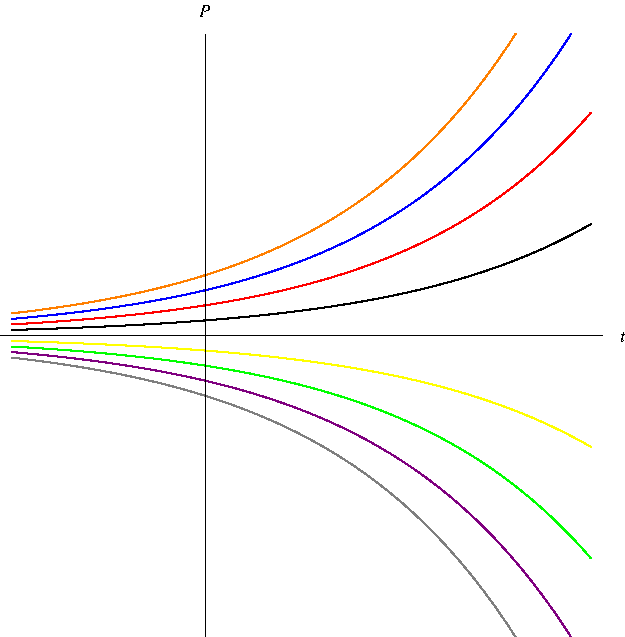
\includegraphics[height=4cm]{diff-eq-models/pictures/10-01-natgrowthb.pdf}%
%}%
%\only<11->{%
%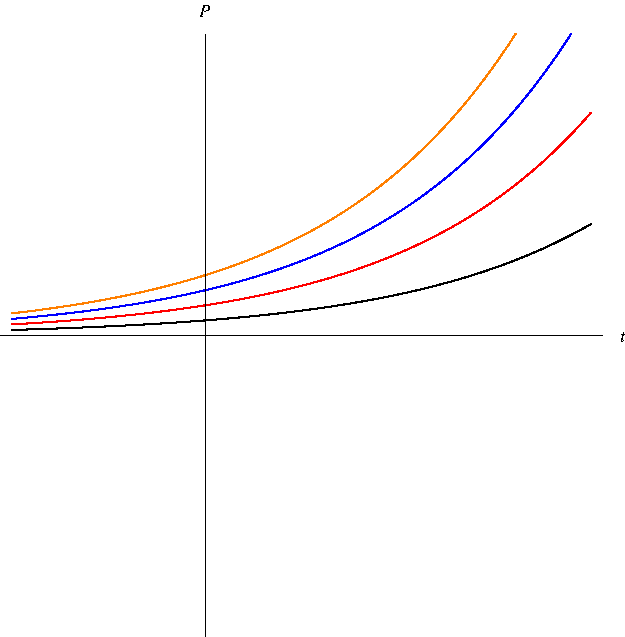
\includegraphics[height=4cm]{diff-eq-models/pictures/10-01-natgrowthc.pdf}%
%}%
\end{columns}
\begin{itemize}
\item  This is a differential equation.
\item<2->  Exponential functions satisfy this condition.
\item<3->  Let $\alert<handout:0| 8>{P(t) = Ce^{kt}}$ ($C$ is a constant).  Then
\abovedisplayskip=0pt
\belowdisplayskip=0pt
\[
\uncover<4->{%
\frac{\diff P}{\diff t} = %
}%
\uncover<5->{%
\frac{\diff}{\diff t} (Ce^{kt}) = %
}%
\uncover<6->{%
 Cke^{kt} = %
}%
\uncover<7->{%
 k\alert<handout:0| 8>{Ce^{kt}} = %
}%
\uncover<8->{%
 k\alert<handout:0| 8>{P(t)} %
}%
\]
\item<9->  Therefore any function of the form $P(t) = Ce^{kt}$ satisfies the equation.  We will see later that there is no other solution.
\item<10->  Letting $C$ vary over the real numbers gives a family of solutions.
\item<11->  Since populations are non-negative, only solutions with $C > 0$ are relevant.
\end{itemize}
\end{frame}
% end module diff-eq-natural-growth-solution
